%% abtex2-modelo-relatorio-tecnico.tex, v-1.7.1 laurocesar
%% Copyright 2012-2013 by abnTeX2 group at http://abntex2.googlecode.com/ 
%%
%% This work may be distributed and/or modified under the
%% conditions of the LaTeX Project Public License, either version 1.3
%% of this license or (at your option) any later version.
%% The latest version of this license is in
%%   http://www.latex-project.org/lppl.txt
%% and version 1.3 or later is part of all distributions of LaTeX
%% version 2005/12/01 or later.
%%
%% This work has the LPPL maintenance status `maintained'.
%% 
%% The Current Maintainer of this work is the abnTeX2 team, led
%% by Lauro César Araujo. Further information are available on 
%% http://abntex2.googlecode.com/
%%
%% This work consists of the files abntex2-modelo-relatorio-tecnico.tex,
%% abntex2-modelo-include-comandos and abntex2-modelo-references.bib
%%

% ------------------------------------------------------------------------
% ------------------------------------------------------------------------
% abnTeX2: Modelo de Relatório Técnico/Acadêmico em conformidade com 
% ABNT NBR 10719:2011 Informação e documentação - Relatório técnico e/ou
% científico - Apresentação
% ------------------------------------------------------------------------ 
% ------------------------------------------------------------------------

% Alterado por Rodrigo Campiolo para apresentação de relatórios na disciplina
% de Redes de Computadores II do Bacharelado em Ciência da Computação da UTFPR-CM.


\documentclass[
	% -- opções da classe memoir --
	12pt,				% tamanho da fonte
	%openright,			% capítulos começam em pág ímpar (insere página vazia caso preciso)
	oneside,   	        % para impressão em verso e anverso use twoside. Oposto a oneside
	a4paper,			% tamanho do papel. 
	% -- opções da classe abntex2 --
	%chapter=TITLE,		% títulos de capítulos convertidos em letras maiúsculas
	%section=TITLE,		% títulos de seções convertidos em letras maiúsculas
	%subsection=TITLE,	% títulos de subseções convertidos em letras maiúsculas
	%subsubsection=TITLE,% títulos de subsubseções convertidos em letras maiúsculas
	% -- opções do pacote babel --
	english,			% idioma adicional para hifenização
	french,				% idioma adicional para hifenização
	spanish,			% idioma adicional para hifenização
	brazil,				% o último idioma é o principal do documento
	]{pacotes/abntex2}


% ---
% PACOTES
% ---

% ---
% Pacotes fundamentais 
% ---
\usepackage{cmap}				% Mapear caracteres especiais no PDF
\usepackage{lmodern}			% Usa a fonte Latin Modern
\usepackage[T1]{fontenc}		% Selecao de codigos de fonte.
\usepackage[utf8]{inputenc}		% Codificacao do documento (conversão automática dos acentos)
\usepackage{indentfirst}		% Indenta o primeiro parágrafo de cada seção.
\usepackage{color}				% Controle das cores
\usepackage{graphicx}			% Inclusão de gráficos
\usepackage{url}
\usepackage[center]{caption}
\usepackage{listings}
% ---

% ---
% Pacotes adicionais, usados no anexo do modelo de folha de identificação
% ---
\usepackage{multicol}
\usepackage{multirow}
% ---
	
% ---
% Pacotes adicionais, usados apenas no âmbito do Modelo Canônico do abnteX2
% ---
\usepackage{lipsum}				% para geração de dummy text
% ---

% ---
% Pacotes de citações
% ---
\usepackage[brazilian,hyperpageref]{backref}	 % Paginas com as citações na bibl
\usepackage[alf]{pacotes/abntex2cite}	% Citações padrão ABNT
\usepackage{comment}
% --- 
% CONFIGURAÇÕES DE PACOTES
% --- 

% ---
% Configurações do pacote backref
% Usado sem a opção hyperpageref de backref
\renewcommand{\backrefpagesname}{Citado na(s) página(s):~}
% Texto padrão antes do número das páginas
\renewcommand{\backref}{}
% Define os textos da citação
\renewcommand*{\backrefalt}[4]{
	\ifcase #1 %
		Nenhuma citação no texto.%
	\or
		Citado na página #2.%
	\else
		Citado #1 vezes nas páginas #2.%
	\fi}%
% ---

% ---
% Informações de dados para CAPA e FOLHA DE ROSTO
% ---
\titulo{Avaliação empírica de algoritmos}
\autor{Cláudia L. Poiet Sampedro\\Igor N. Faustino\\João Victor Nascimento\\Letícia Mazzo Portela}
\local{Campo Mourão}
\data{Novembro / 2017}
\instituicao{%
  Universidade Tecnológica Federal do Paraná -- UTFPR
  \par
  Departamento Acadêmico de Computação -- DACOM
  \par
  Bacharelado em Ciência da Computação -- BCC
}
\tipotrabalho{Relatório técnico}
% O preambulo deve conter o tipo do trabalho, o objetivo, 
% o nome da instituição e a área de concentração 
\preambulo{Relatório técnico de atividade prática solicitado pelo professor Rodrigo Campiolo na disciplina de Análise de Algoritmos do Bacharelado em Ciência da Computação da Universidade Tecnológica Federal do Paraná.}
% ---

% ---
% Configurações de aparência do PDF final

% alterando o aspecto da cor azul
\definecolor{blue}{RGB}{41,5,195}

% informações do PDF
\makeatletter
\hypersetup{
     	%pagebackref=true,
		pdftitle={\@title}, 
		pdfauthor={\@author},
    	pdfsubject={\imprimirpreambulo},
	    pdfcreator={LaTeX with abnTeX2},
		pdfkeywords={abnt}{latex}{abntex}{abntex2}{relatório técnico}, 
		colorlinks=true,       		% false: boxed links; true: colored links
    	linkcolor=blue,          	% color of internal links
    	citecolor=blue,        		% color of links to bibliography
    	filecolor=magenta,      		% color of file links
		urlcolor=blue,
		bookmarksdepth=4
}
\makeatother
% --- 

% --- 
% Espaçamentos entre linhas e parágrafos 
% --- 

% O tamanho do parágrafo é dado por:
\setlength{\parindent}{1.3cm}

% Controle do espaçamento entre um parágrafo e outro:
\setlength{\parskip}{0.2cm}  % tente também \onelineskip

% ---
% compila o indice
% ---
\makeindex
% ---

% Omite a numeração de capítulos
\renewcommand*\thesection{\arabic{section}}



% ----
% Início do documento
% ----
\begin{document}

% Retira espaço extra obsoleto entre as frases.
\frenchspacing 

% ----------------------------------------------------------
% ELEMENTOS PRÉ-TEXTUAIS
% ----------------------------------------------------------
% \pretextual

% ---
% Capa
% ---
%\imprimircapa
% ---

% ---
% Folha de rosto
% (o * indica que haverá a ficha bibliográfica)
% ---
\imprimirfolhaderosto
% ---


% ---
% RESUMO
% ---

% resumo na língua vernácula (obrigatório)
\begin{resumo}
 Desde agosto de 2017 foram expostos diversos conceitos na disciplina de Análise de Algoritmos, tendo esta importância elevada, já que é caracterizada como fundamental na área de Computação. Em vista disso, o presente trabalho contempla aplicações práticas dos conceitos vistos em sala de aula, especificamente, na análise empírica de algoritmos. Para tal feito, foram realizadas comparações, em quatro linguagens de programação diferentes, de quatro versões do algoritmo Subvetor Máximo. Dessa forma, pretende-se mostrar como o comportamento de um mesmo algoritmo pode variar, levando em conta a linguagem em que foi elaborado, o hardware em que foi executado, o software utilizado e, também, certas configurações específicas. 

 \vspace{\onelineskip}
    
 \noindent
 \textbf{Palavras-chave}: Análise empírica. Algoritmos. Linguagens de programação.
\end{resumo}
% ---

% ---
% inserir lista de ilustrações
% ---
%\pdfbookmark[0]{\listfigurename}{lof}
%\listoffigures*
%\cleardoublepage
% ---

% ---
% inserir lista de tabelas
% ---
%\pdfbookmark[0]{\listtablename}{lot}
%\listoftables*
%\cleardoublepage
% ---

% ---
% inserir lista de abreviaturas e siglas
% ---
%\begin{siglas}
%  \item[IP] Internet Protocol
%  \item[TCP] Transmission Control Protocol
%  \item[UDP] User Datagram Protocol
%\end{siglas}
% ---

% ---
% inserir o sumario
% ---
\pdfbookmark[0]{\contentsname}{toc}
\tableofcontents*
\cleardoublepage
% ---

% ----------------------------------------------------------
% ELEMENTOS TEXTUAIS
% ----------------------------------------------------------
\textual

\makeatletter
\renewcommand{\chapter}{\@gobbletwo}
\makeatother

\section{Introdução}
\label{sec:introducao}
    Os algoritmos têm por finalidade resolver problemas por meio de uma sequência bem definida de ações, sendo possível existir diversos algoritmos, elaborados de formas diferentes, para resolver o mesmo problema. Em vista disso, existe a Análise de Algoritmos, cujo propósito é o de fazer uma previsão dos recursos que determinado algoritmo fará uso \cite{art5}. Assim, ao contrapor dois algoritmos que resolvem o mesmo problema, é possível determinar, através da Análise de Algoritmos, qual deles é o mais eficiente, levando em conta fatores como tempo de execução, quantidade de entradas, dentre outros.
    
    Ao longo do segundo semestre de 2017, foram abordados diversos conceitos e demonstrados exemplos na disciplina de "Análise de Algoritmos", ministrada pelo professor Rodrigo Campiolo, no quarto período do curso de Bacharelado em Ciência da Computação. Sendo assim, com base no que fora apresentado, solicitou-se a elaboração do presente relatório, no qual se encontram considerações a respeito da avaliação empírica de algoritmos.
    
    Assim, para a elaboração do respectivo relatório, foi tomado como base o Problema do Subvetor Máximo. Para resolver tal problema, foram apresentadas quatro maneiras: Enumeração, Enumeração Melhorada, Divisão e Conquista, e Programação Dinâmica \cite{art6}.
    
    Para tanto, solicitou-se que para cada maneira de se resolver o problema, fossem desenvolvidas quatro versões em linguagens de programação diferentes, sendo exigido que pelo menos uma dessas linguagens fosse compilada e pelo menos uma interpretada. Dessa forma, as linguagens escolhidas foram: C (compilada), Pascal (compilada), Java (interpretada) e Python (interpretada). Em seguida, realizou-se a análise empírica dos algoritmos desenvolvidos.

\section{Objetivos}
\label{sec:objetivos}
    Como mencionado na seção anterior, o presente relatório tem como intuito aplicar o conhecimento que fora adquirido em sala de aula. Além disso, por meio da análise empírica, pretende-se mostrar como o comportamento de um mesmo algoritmo pode variar, levando em conta a linguagem em que foi elaborado, o hardware em que foi executado, o software utilizado e, também, certas configurações específicas. 

\section{Fundamentação}
\label{sec:fundamentacao}
    \subsection{Análise Empírica}
        A análise empírica ou avaliação empírica de algoritmos, se caracteriza como o estudo do tempo despendido para a execução de certos algoritmos. A medição deste tempo pode ser realizada através da contagem do número de vezes que cada instrução presente no código em questão é executada ou pela temporização de cada trecho do algoritmo \cite{art8}.
        Assim, por meio dos procedimentos citados, é possível efetuar a otimização do algoritmo, pois se consegue localizar os pontos em que leva mais tempo para executar.
        
        Importante salientar que o hardware e software utilizados na execução do algoritmo, além de determinadas configurações, são influenciadores para o tempo de execução despendido pelo mesmo e, também, para a forma com que será utilizada a memória.
        
        Sendo assim, segundo Fabro (2009), os principais objetivos da análise empírica são: "avaliar a corretude dos algoritmos, comparar a eficiência de diferentes algoritmos, comparar implementações alternativas do mesmo algoritmo, identificar a complexidade do algoritmo".
    
    \subsection{Problema do Subvetor Máximo}
        Seja um vetor \textit{V[1..n]} com \textit{n} números inteiros positivos e negativos, o subvetor \textit{V[e..d]}, em que \textit{e >= 1}, \textit{d <= n} e $\sum_{i=e}^{d}$ \textit{V[i]}
        é máxima, é denominado subvetor máximo \cite{art7}.
        
        Por exemplo, dado o vetor \textit{V[31, -41, \textbf{59}, \textbf{26}, \textbf{-53}, \textbf{58}, \textbf{97}, -93, -23, 84]}, a soma dos elementos em destaque é igual a 187, sendo o subvetor máximo, portanto, identificado por estes elementos.
    
    \subsection{Linguagens de Programação}
        \subsubsection{C}
            A linguagem de programação C foi criada em 1970 por Dennis Ritchie, no AT&T Bell Labs, nos Estados Unidos. Sua criação foi baseada na linguagem B, criada por Ken Thompson \cite{art2}.
            
            C se caracteriza como uma linguagem estruturada, assim sendo, é necessário que os programas desenvolvidos nessa linguagem sigam uma disciplina, facilitando sua correção. Além disso, C é \textit{case sensitive}, ou seja, diferencia letras maiúsculas de minúsculas.
        
        \subsubsection{Pascal}
            Pascal é uma linguagem de programação criada em 1968 por Niklaus Wirth, do Instituto de Informática ETH (Eidgenossische Technische Hochschule), em Zurique, Suiça. Seu nome é uma homenagem ao matemático Blaise Pascal (1623-1662) e, além disso, foi criada tendo como base as linguagens ALGOL e PL/I \cite{art1}.
            
            Assim como C, Pascal também é considerada uma linguagem de paradigma estruturado. Todavia, devido ao fato de ter surgido antes de C, é reconhecida como uma linguagem que revolucionou o que se conhecia por linguagens de programação até então, por conta dos novos conceitos que trouxe, bem como criação de novos tipos, uso de funções e procedimentos recursivos, etc. \cite{art1}.
        
        \subsubsection{Java}
            A linguagem Java teve sua primeira versão lançada em 1996, no entanto, começou a ser elaborada em 1991 em alguns projetos de um grupo de funcionários da Sun Microsystems (hoje pertencente a Oracle Corporation), nos Estados Unidos. Seu nome é uma homenagem às xícaras de café, já que a equipe, durante o seu desenvolvimento, ingeria muito café \cite{art3}.
            
            Java foi utilizada, inicialmente, no ambiente web, onde obteve grande sucesso. Com o tempo, passou por várias evoluções e nos dias atuais é utilizada em diversas aplicações e dispositvos presentes no cotidiano \cite{art3}. Vale ressaltar que o paradigma utilizado por essa linguagem é o de orientação a objetos, onde os principais conceitos utilizados são os de Classes, Objetos, Associação e Encapsulamento.
        
        \subsubsection{Python}
            Python é uma linguagem de programação que foi criada em 1982 por Guido Van Rossun, no CWI (Centrum Wiskund \& Informatica), em Amsterdâ, Holanda. Essa linguagem foi desenvolvida com o intuito de sempre possuir liberdade, ser gratuita e de código aberto, além de ter disponibilidade para vários sistemas e possuir clareza em sua sintaxe \cite{art4}.
            
            Da mesma forma que Java, Python também se enquadra no paradigma de orientação a objetos e, além disso, possui alta modularidade. Um fato interessante a respeito dessa linguagem, é que a mesma já foi utilizada pela empresa Industrial Lights and Magic para realizar o controle de certos efeitos de Star Wars, dentre outras aplicações \cite{art4}.

\section{Materiais}
\label{sec:materiais}
    Para a execução e avaliação dos algoritmos, foi utilizado um notebook com processador Intel Core i7 com velocidade de 2.2GHz, 8GB de memória RAM e 1TB de disco rígido. Além disso, o sistema operacional era o Linux Debian versão 9.

\section{Procedimentos}
\label{sec:procedimentos}
    Como previamente citado e referenciado, foram implementadas quatro formas do mesmo algoritmo em quatro linguagens, as quais possuem complexidade e tempo de execução distintos \cite{art6}. Todos os códigos foram testados com 5 entradas díspares, entretanto, estas possuem a mesma semente de inicialização. Além disso, foi usada uma função para gerar números aleatórios, e estes foram salvos em arquivos. Todos os códigos e linguagens foram providos dos mesmos arquivos gerados, os quais possuíam entradas de 500, 1000, 2500, 5000 e 7500 dados.
    
    A primeira versão do algoritmo, chamada de Enumeração, percorria com um laço de repetição a cada par do vetor, executando a soma e mantendo esta salva. A cada iteração dos laços, a soma anterior era comparada a atual, sendo armazenado o maior valor entre elas. Este algoritmo possui complexidade T(n) = O(n³), sendo bastante custoso e delongado quando executado com entradas robustas.
    
    A segunda implementação mantinha a mesma lógica da anterior, entretanto, eliminava o laço que percorria cada par e, por consequência, a soma não era computada tantas vezes. Este algoritmo possui complexidade T(n) = O(n²), caracterizando-se como mais viável do que o anterior. 
    
    Na terceira implementação foi tirado proveito do conceito de Divisão e Conquista, o qual consiste em dividir o vetor em partes menores, para facilitar o processamento, e juntar as mesmas depois de processadas, chegando ao resultado desejado. No caso deste algoritmo, ao dividir o vetor existe a possibilidade da soma máxima estar na primeira ou segunda metade, ou então, entre estas. Esta versão possui complexidade T(n) = O(nlgn).
    
    A ultima versão implementada usava programação dinâmica como base, partindo da premissa que o subvetor máximo usa ou não o último elemento do vetor principal. Esta é a implementação menos custosa, possuindo complexidade T(n) = O(n).
    
 
\section{Discussão dos Resultados}
\label{sec:discussao}
    
    Os resultados das comparações entre os algoritmos foram reunidos em gráficos, os quais relacionam o tamanho das entradas com o tempo real de execução, medido em escala logarítmica, apenas da função que encontra o maior subvetor. Para melhor aplicação da análise empírica, foram ignoradas as seções de entrada e saída. 
    
    Cada gráfico retrata uma implementação, usando linhas de cores distintas para representar cada uma das linguagens. No eixo X estão contidos os tamanhos das entradas e no Y o tempo gasto em milissegundos.
    
    \begin{figure}[!htb]
      \centering
      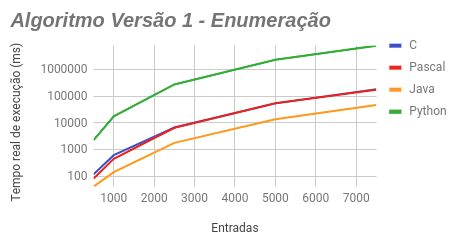
\includegraphics[scale=0.55]{figuras/enumeracao.png}
      \caption{Comparação das linguagens no algoritmo de Versão 1.}
      \label{fig:f1}
    \end{figure}
    
    Na Figura 1, onde está representada a primeira versão, é visível que o algoritmo implementado em Python possui desempenho degradado em relação as outras linguagens utilizadas. Quando esta implementação é executada com entradas robustas, independente da linguagem, é perceptível um considerável prolongamento no tempo de execução. 
    
    A linguagem Java veio a se destacar pelo seu desempenho, mesmo com entradas numerosas mostrou menor tempo de execução quando comparada as outras linguagens testadas. C e Pascal apresentaram desempenho semelhante, expressando tempo médio em relação às outras ferramentas utilizadas.

    
    \begin{figure}[!htb]
      \centering
      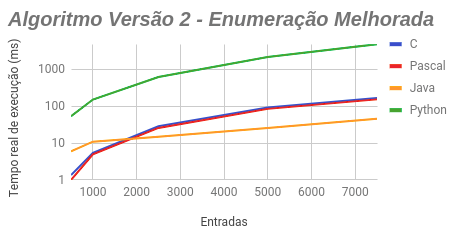
\includegraphics[scale=0.55]{figuras/enumeracao2.png}
      \caption{Comparação das linguagens no algoritmo de Versão 2.}
      \label{fig:f2}
    \end{figure}

     A Figura 2 representa o algoritmo de Enumeração Melhorada. Neste, é visível comportamento próximo ao da Figura 1, quando empregadas entradas numerosas: Python apresentando pior desempenho, Java o melhor, C e Pascal desempenho mediano. Entretanto, é perceptível que nos testes com os menores arquivos, até aproximadamente 1800 entradas, as linguagens C e Pascal se destacam e manifestam um ótimo desempenho.

    \begin{figure}[!htb]
      \centering
      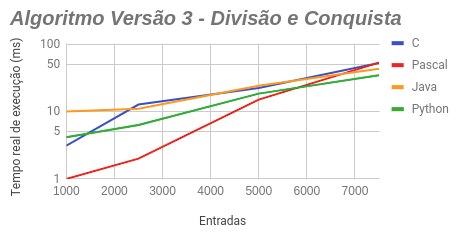
\includegraphics[scale=0.55]{figuras/divisao.png}
      \caption{Comparação das linguagens no algoritmo de Versão 3.}
      \label{fig:f3}
    \end{figure}
    
    O terceiro algoritmo, Divisão e Conquista, está com seus resultados representados pela Figura 3. Nesta, é notável o distinto comportamento das linguagens para entradas pequenas, mas, a medida que estas crescem, os resultados tendem a se parelhar de maneira geral.
    
    Para arquivos pequenos e médios, Pascal situa-se com os melhores resultados, os quais estão relativamente distantes das outras linguagens. As outras 3 implementações não possuem distanciamento de valores tão abruptos, embora Java principie com os piores resultados.
    
    \begin{figure}[!htb]
      \centering
      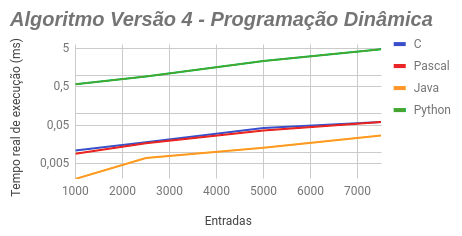
\includegraphics[scale=0.55]{figuras/dinamica.png}
      \caption{Comparação das linguagens no algoritmo de Versão 4.}
      \label{fig:f4}
    \end{figure}
    
    Tendo a Figura 4 como reprodução dos resultados obtidos através da execução do 4º algoritmo, pautado por programação dinâmica, foram obtidos resutados bastante satisfatórios. Assim, devido a complexidade do algoritmo ser T(n) = O(n), mesmo em entradas maiores o tempo se manteve baixo.
    
    Python foi a linguagem com pior desempenho, gastanto 5 milissegundos para a maior entrada, enquanto Java, com o melhor desempenho, levou em média 0,03ms. C e Pascal mantiveram resultados parecidos e com pouca diferença do melhor obtido.
    
\section{Conclusões}
\label{sec:conclusoes}

    Após a analise dos resultados, pode-se concluir que a 1ª versão do algoritmo de SubVetor Máximo é muito custosa e quase inviável para entradas maiores. O pior desempenho nesta versão foi encontrado na implementação em Python, que para uma entrada de 7500 dados levou algo em torno de 2 horas para a execução. O melhor desemenho vem a cargo do Java, que demorou aproximadamente 45 segundos para o processamento da mesma entrada.
    
    A 2ª versão, apesar de melhor que a primeira, também apresenta tempos de execução altos. O padrão das linguagens da primeira versão se mantém, mas é notável que para arquivos de até aproximadamente 1800 entradas, C e Pascal demonstraram melhor comportamento.
    
    A implementação com base em Divisão e Conquista foi a que mais aproximou os resultado das 4 linguagens. Para entradas grandes, todas apresentaram tempo de execução parecido, em torno de 50 milissegundos. Considerando arquivos de até algo próximo a 5000 entradas, Pascal se destaca com os menores tempos.
    
    A ultima versão é a com melhor complexidade (O(n)), rendendo ótimos resultados mesmo para entradas robustas, em todas as linguagens. Entretanto, Python obteve o pior resultado, chegando a apresentar índice de piora de quase 100 vezes para a maior entrada, quando comparado aos resultados medianos, obtidos por C e Pascal.
    
    Se tratando dos algoritmos, conforme foram mudando as versões, sequencialmente, o tempo real de execução foi decrescendo, mas é discrepante a melhora no tempo quando comparada a 1ª com a última versão, independente da linguagem avaliada. 
    
    A respeito das linguagens, de maneira geral, Python se portou com os piores resultados, enquanto Java com os melhores. C e Pascal apresentaram valores bastantes semelhantes e, por várias vezes, medianos em relação as outras duas linguagens escolhidas.
    
    

% ----------------------------------------------------------
% ELEMENTOS PÓS-TEXTUAIS
% ----------------------------------------------------------
\postextual
% ----------------------------------------------------------
% Referências bibliográficas
% ----------------------------------------------------------
\renewcommand{\bibsection}{%
\section{\bibname}
\bibmark
%\ifnobibintoc\else
%\phantomsection
%\addcontentsline{toc}{section}{\bibname}
%\fi
\prebibhook}

\bibliography{abntex2-modelo-references}


\end{document}
